\section{What has actually been measured}
\label{sec:measured}

\begin{figure*}[t]
\centering
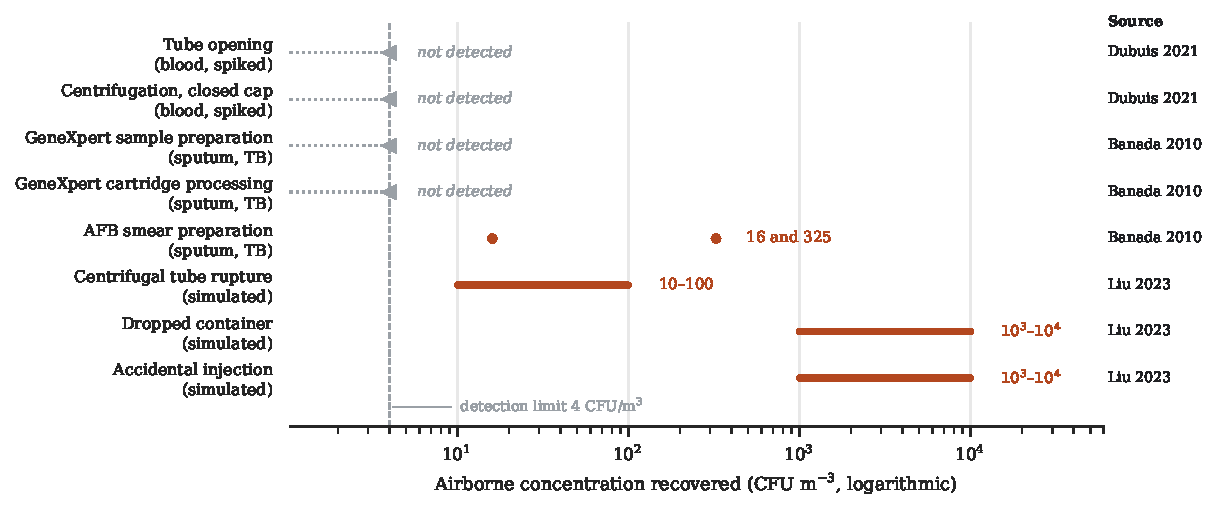
\includegraphics[width=0.96\textwidth]{figures/fig1_measured_concentrations.pdf}
\caption{Every airborne concentration measurement located for clinical
laboratory bench work, on one logarithmic axis. Four conditions yielded no
recoverable organisms; for the two blood-handling conditions the reported
detection limit was 4~CFU\,m$^{-3}$. Acid-fast smear preparation yielded two
discrete values, 16 and 325~CFU\,m$^{-3}$, plotted individually rather than as
a range. The three simulated accident conditions were measured in a research
biosafety laboratory using 30~mL of concentrated suspension, not clinical
specimens. The studies were not designed to be compared and differ in
organism, sampler, room and specimen; the axis shows what exists, not a
calibrated ranking.}
\label{fig:measured}
\end{figure*}

Figure~\ref{fig:measured} assembles every airborne concentration measurement
located for bench work of the kind this inventory covers. Three observations
follow from it, and the first is simply how short the list is.

\subsection{Four conditions in which nothing was recovered}

Two pre-analytical blood-handling conditions, tube opening and closed-cap
centrifugation, yielded no recoverable organisms down to 4~CFU\,m$^{-3}$
\cite{dubuis2021}. Two tuberculosis molecular testing conditions, sample
preparation and automated cartridge processing, yielded no culturable
bioaerosol \cite{banada2010}.

These four negatives carry most of the reassurance available in the current
evidence base, and they must be read with their conditions attached. The
blood-handling measurements were made with closed-cap tubes in a swing-bucket
rotor and with tube opening performed behind a plexiglass panel. They are
evidence that those containment arrangements work. Read as evidence that an
unprotected bench is safe, they say something the study did not test. A
detection limit of 4~CFU\,m$^{-3}$ is also not zero, and for an organism with
a low inhaled infectious dose the distinction is not academic.

\subsection{The one before-and-after comparison}

Banada and colleagues measured viable bioaerosol at each stage of the
cartridge-based tuberculosis assay workflow and, in the same study, during
preparation of smears for acid-fast microscopy \cite{banada2010}. The assay
stages produced no culturable bioaerosol. Smear preparation produced 16 and
325~CFU\,m$^{-3}$.

This is the only place in the inventory where one procedure was measured
against the procedure it displaces, under comparable conditions, in one study.
It is discussed further in Section~\ref{sec:tb}.

\subsection{The accident measurements, and their ordering}

Liu and colleagues measured source intensities for three simulated high-risk
procedures \cite{liu2023}. Centrifugal tube rupture fell at roughly 10 to
100~CFU\,m$^{-3}$; dropped containers and accidental injection fell at roughly
$10^{3}$ to $10^{4}$~CFU\,m$^{-3}$, two orders of magnitude higher.

The ordering is the useful part and it runs against intuition. Centrifuge
accidents dominate discussion of pre-analytical biosafety; in the one study
that measured them alongside other accident types, they were the least intense
of the three. A dropped specimen container, which is the characteristic
accident of the receiving area rather than the centrifuge room, was measured
far higher.

The magnitudes should not be transferred to clinical settings. That work used
30~mL of concentrated suspension in a research biosafety laboratory, a quantity
and concentration unlike a routine clinical specimen. The inventory therefore
grades specimen reception \textbf{E2}, flagging the inference, rather than E1.

\subsection{What the figure does not support}

The studies in Figure~\ref{fig:measured} were not designed to be compared.
They differ in organism, in sampler type and flow rate, in room ventilation,
in specimen matrix and in whether the material was a spiked surrogate or a
patient specimen. No formal cross-study comparison is warranted, and none is
offered.

What the figure does support is a statement about coverage. Of seven routine
bench steps, measurements exist for parts of three. There is no measurement at
all for automated analyser operation, for MALDI-TOF target preparation, or for
open-bench subculture, and the last two of those are the steps with documented
human infections.
